上ではbeegoフレームワークにおいてcontroller基底クラスの設計を完成させました。我々のアプリケーションでは我々のメソッドを以下のように設計することができます:

\begin{lstlisting}[numbers=none]
package controllers

import (
    "github.com/astaxie/beego"
)

type MainController struct {
    beego.Controller
}

func (this *MainController) Get() {
    this.Data["Username"] = "astaxie"
    this.Data["Email"] = "astaxie@gmail.com"
    this.TplNames = "index.tpl"
}
\end{lstlisting}

上のメソッドではサブクラスMainControllerを実装し、Getメソッドを実装しています。もしユーザがその他のメソッド(POST/HEAD等)によってこのリソースにアクセスすると、403を返します。もしGetであれば、AutoRender=trueを設定していますのでGetメソッドの実行後自動的にRender関数が実行され、以下のようなインターフェースが表示されます:

\begin{figure}[H]
   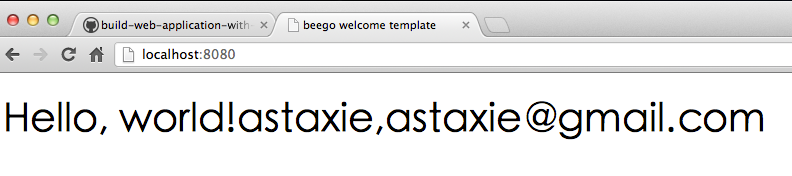
\includegraphics[width=14cm]{13.4.beego.png}
   \label{}
   \caption{}
\end{figure}

index.tplのコードは以下のようになります。データの設定と表示が非常に簡単になっていることが見てとれます:

\begin{lstlisting}[numbers=none]
<!DOCTYPE html>
<html>
  <head>
    <title>beego welcome template</title>
  </head>
  <body>
    <h1>Hello, world!{{.Username}},{{.Email}}</h1>
  </body>
</html>
\end{lstlisting}

